\chapter{Gestion des variations} % Main chapter title

\label{Chapitre3} % For referencing the chapter elsewhere, use \ref{Chapter1} 
\lhead{Chapitre 3. \emph{Gestion des variations}} % This is for the header on each page - perhaps a shortened title
Une variation est considéré comme toute action non définie dans le modèle de procédé initiale ou qui viole certaines contraintes de procédés.
Après une étude de l'existant, nous allons proposer deux solutions de gestion de variations. La première solution consiste à traiter les variations grâce à un PSEE; la seconde solution quand à elle, utilise un fichier excel pour gérer les variations.
Alors cette partie sera composée de nos techniques de détection de variations (la technique à l'aide d'un PSEE et la seconde technique à l'aide d'un fichier excel).
\section{Solution 1}
Comme nous l'avons dit dans le chapitre~\ref{Chapitre2}, l'OMG a proposé en 2005 le SPEM 1.1, mais ce dernier présentant quelques lacunes, ils ont proposé en 2008 une nouvelle version (SPEM 2.2). 
Ces normes de l'OMG sont utilisés dans de nombreux travaux de recherches car ils sont considérés aujourd'hui comme étant un modèle assez complet pour pouvoir décrire les procédés. Alors pour cette première solution, je me suis beaucoup basé sur les solutions proposées par l'OMG dans leurs travaux.
\subsection{Méta-modèle de procédé}
Avant d'expliquer la technique de détection, nous allons définir notre méta-modèle de procédé c'est à dire notre modèle définissant les concepts de base d'un langage de description de procédés.
La figure~\ref{metamodele} représente notre méta-modèle de procédé. Nous avons récupéré les éléments importants proposés par l'OMG et avons rajouter nos éléments pour nous permettre de détecter et de corriger les variations.

\begin{figure}[h]
\centering
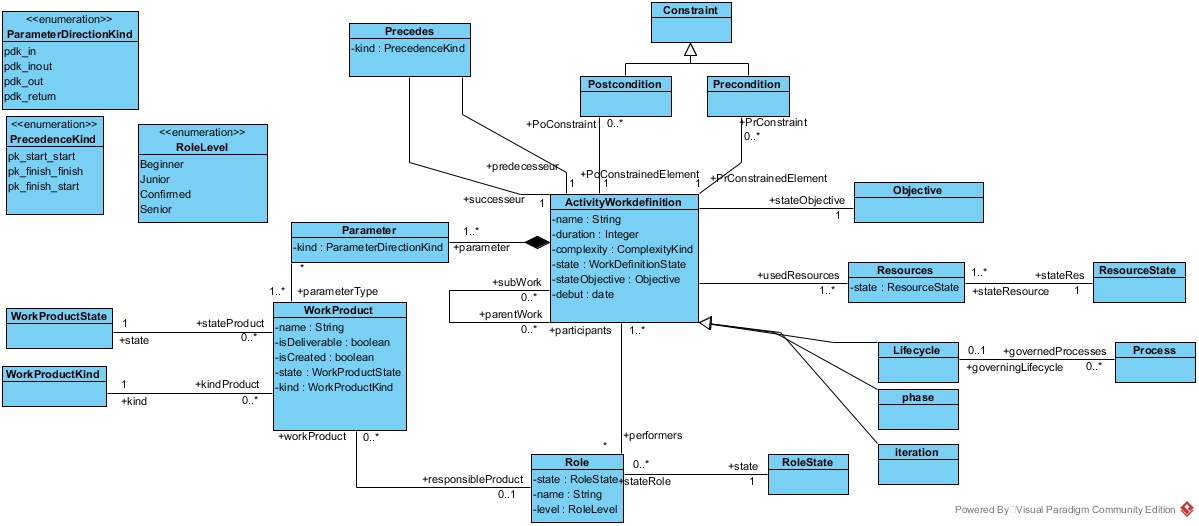
\includegraphics[width=16cm]{Solution.jpg}
\caption{\label{metamodele}Méta-modèle de SPEM solution}
\end{figure}

Nous allons maintenant décrire chaque élément de notre méta-modèle.
\subsubsection*{ActivityWorkDefinition}
L'élément \textbf{\textit{ActivityWorkDefinition}} représente un travail ou une tâche à réaliser durant le processus de développement logiciel. Ces tâches doivent être réalisées par des acteurs décrits par \textit{Role} pendant une durée donnée.\\
Les attributs de cet élément sont:\\
\begin{itemize}
\item[\tiny{$\blacksquare$}] Name: c'est une chaine de caractère qui correspond au nom de la tâche.
\item[\tiny{$\blacksquare$}] State: de type \textit{ActivityWorkDefinitionState}, il permet de connaitre l'état de la tâche.
\item[\tiny{$\blacksquare$}] Duration: nombre représentant la durée de la tâche.
\item[\tiny{$\blacksquare$}] Complexity: indique le niveau de difficulté ou le degré de complexité de la tâche. Il pourra nous être utile pendant le traitement d'une déviation.
\item[\tiny{$\blacksquare$}] stateObjective: attribut de type \textit{Objective}, il indique l'objectif ou le but du travail.
\end{itemize}
\subsubsection*{WorkProduct, WorkProductKind, WorkProductState}
L'élément \textbf{\textit{WorkProduct}} ou artéfact représente tout ce qui est produit, modifié ou consommé par un \textit{ActivityWorkDefinition}. Ses attributs sont:\\
\begin{itemize}
\item[\tiny{$\blacksquare$}] Name: chaine de caractère représentant le nom du produit.
\item[\tiny{$\blacksquare$}] isDeliverable: booléen permettant de savoir si le produit peut être délivré ou pas.
\item[\tiny{$\blacksquare$}] Kind: de type \textit{WorkProductKind}, il permet de connaitre le type du produit c'est à dire si c'est un document, model ou code.
\item[\tiny{$\blacksquare$}] State: indique l'état du produit, il est de type \textit{WorkProductState}.
\item[\tiny{$\blacksquare$}] isCreated: booléen permettant de savoir si le produit fut crée ou pas par la tâche.
\end{itemize}
Un \textbf{\textit{WorkProductKind}} représente les catégories de produits que l'on peut avoir. Ces catégories peuvent être du code, des documents, du model etc.\\
L'élément \textit{WorkProductState} indique les états d'un produit (initial, validé, invalidé etc...)

\subsubsection*{RoleLevel, Role}
\textit{RoleLevel} est une énumération des niveaux qu'un rôle peut avoir (débutant, junior, confirmé, senior).\\
Un \textit{Role} représente les rôles ou acteurs responsables d'un produit ou contribuant à la réalisation d'une tâche. Par exemple on peut avoir des analystes, des testeurs etc... Cet élément rôle possède un attribut \textit{name} qui indique le nom du rôle;  un attribut \textit{state} indiquant l'état du rôle c'est à dire si le rôle a terminé d'accomplir la tâche ou si il est en train de le faire etc... et un attribut \textit{level} qui indique le niveau de l'acteur (débutant, junior, confirmé). 
\subsubsection*{Postcondition et Precondition}
Les éléments \textbf{\textit{Precondition}} et \textbf{\textit{Postcondition}} sont des spécialisation de la classe \textit{Constraint}. Il représentent respectivement les conditions qui doivent être satisfaites avant et après l'exécution de chaque \textit{ActivityWorkDefinition}. 
\subsubsection*{Parameter}
L'élément \textbf{\textit{Parameter}} est composé d'un attribut \textit{kind} de type \textbf{\textit{ParameterDirectionKind}} qui est une énumération des types de relations qui relie une tâche à un produit. C'est à dire qu'il permet d'indiquer si un \textit{WorkProduct} est utilisé par une \textit{ActivityWorkDefinition} tant que \og entrée \fg{}, \og sortie \fg{} ou \og entrée/sortie \fg{}. 
\subsubsection*{Precedes et PrecedenceKind}
Pour expliquer les relations qui lient nos \textit{ActivityWorkDefinition}, nous allons prendre deux tâches t1 et t2, t2 étant le successeur de t1.
L'élément \textbf{\textit{PrecedenceKind}} est une énumération des relations qui peuvent exister entre nos \textit{ActivityWorkDefinition}: 
\textit{pk\_start\_start}: ce type de relation permet d'indiquer que t2 ne pourra commencer que si t1 commence.\\
\textit{pk\_finish\_finish}: ce type de relation permet d'indiquer que t2 ne pourra terminer que si t1 l'est.\\
\textit{pk\_finish\_start}: indique que t2 ne pourra commencer qu'à la fin de t1.\\
L'élément \textbf{\textit{Precedes}} comporte un attribut \textit{kind} de type \textit{PrecedenceKind}, il indique le type d'ordonnancement qui relie les \textit{ActivityWorkDefinition}. Par exemple supposons que nos deux tâches t1 et t2 sont reliées par une liaison de type pk\_start\_start, t2 ne peut pas commencer tant que t1 n'a pas commencé.
\subsubsection*{Objective}
L'élément \textbf{\textit{Objective}} représente l'objectif ou le but de la réalisation d'une tâche. Si une tâche est terminée, on pourra vérifier si l'objectif a été atteint.
\subsubsection*{ResourceState, Resources}
\textit{ResourceState} représente les états de disponibilités des ressources.
L'élément \textbf{\textit{Ressources}} représente les différentes ressources. Ces ressources sont utilisées par des tâches selon leurs disponibilités.
\subsubsection*{LifeCycle, Phase, Iteration}
L'élément \textbf{\textit{LifeCycle}} représente le cycle de vie de logiciel par exemple\og le modèle cascade \fg{} ou\og le modèle en V\fg{}
La \textbf{\textit{Phase}} est une spécialisation de \textit{ActivityWorkDefinition}. C'est une tâche correspondant à une phase d'un cycle de vie de logiciel 
L'élément \textbf{\textit{Iteration}} est une \textit{ActivityWorkDefinition} avec des préconditions et objectif bien défini appelé \og minor milestone \fg{}.
%\subsection{Well-formedness rules}
%Nous allons donner ci-dessous la traduction en OCL de nos éléments décrits ci-dessus.
\subsection{Technique de détection des variations et guide de correction}
Cette partie explique la technique de détection des variations et les solutions pour les résoudre.
%\begin{itemize}
%\item[\tiny{$\blacksquare$}]\textbf{ActivityWorkDefinition}
%\item[\tiny{$\blacksquare$}]\textbf{WorkProduct}
%\item[\tiny{$\blacksquare$}]\textbf{Postcondition}
%\item[\tiny{$\blacksquare$}]\textbf{Precondition}
%\item[\tiny{$\blacksquare$}]\textbf{Parameter}
%\item[\tiny{$\blacksquare$}]\textbf{Precedes}
%\item[\tiny{$\blacksquare$}]\textbf{Objective}
%\item[\tiny{$\blacksquare$}]\textbf{ResourceState}
%\item[\tiny{$\blacksquare$}]\textbf{Resources}
%\item[\tiny{$\blacksquare$}]\textbf{LifeCycle}
%\item[\tiny{$\blacksquare$}]\textbf{Phase}
%\item[\tiny{$\blacksquare$}]\textbf{Iteration}
%\item[\tiny{$\blacksquare$}]\textbf{RoleState}
%\item[\tiny{$\blacksquare$}]\textbf{Role}
%\item[\tiny{$\blacksquare$}]\textbf{Process}
%\end{itemize}
\subsubsection*{Technique de détection}
Rappelons nous qu'une variation est toute actions qui violent les contraintes définis dans notre procédé.
Alors, notre technique de détection des variations est simple, elle se base sur certains attributs de notre modèle.
Ces attributs sont tous les attributs représentant des contraintes. On surveille l'exécution des procédés, avant chaque exécution, on vérifie si les conditions requises pour commencer la tâche sont satisfaites c'est à dire si la pré-condition est satisfaite, si les relations de précédence sont également satisfaite. A la fin de chaque exécution, on vérifie si les post-conditions sont remplis, si la tâche est correctement terminée et l'objectif du travail est atteint. Si on voit qu'il y'a une anomalie au niveau de la satisfaction de nos contraintes alors on signale une déviation et on propose un plan de correction au chef de projet.
\subsubsection*{Guide de correction}
Notre technique de correction est basé sur la ré-exécution de la tâche ou peut-être l'ignorer. Si une déviation est détectée, on regarde les causes ensuite on propose au chef de projet les solutions suivantes:\\
\begin{itemize}
\item[\tiny{$\blacksquare$}] ignorer la déviation si elle est mineure comme par exemple, on veut lancer une tâche dont toutes les pré-conditions sont satisfaites mais la date supposé être la date de lancement de la tâche n'est pas arrivé, alors on peut proposer au chef de projet de modifier la date ou de l'ignorer. Car ça ne va pas générer des erreurs négatives (comme un retard dans la livraison).
\item[\tiny{$\blacksquare$}] la seconde solution à analysé les causes:\\
si c'est un dépassement de la date limite du travail, on pourra proposer au chef de projet d'affecter la tâche à un rôle plus compétent si le rôle responsable de la tâche n'est pas assez compétent sinon on modifie la date limite et on laisse le même rôle continuer à exécuter la tâche. Sinon si c'est l'exécution d'une action non défini dans le modèle de procédé initial, on demande au chef de projet de redéfinir le modèle de procédé.
\end{itemize}
\section{Deuxième solution}
Pour cette deuxième solution, je me suis rapproché d'un chef de projet chez \og Alstom \fg{} afin de mettre en place cette solution. C'est une solution plus simple car elle est réalisée à l'aide d'un fichier excel.
